\scanpage{14}
\textcircled{4}\quad Supposons que $\mathfrak g=L_k(M)$, où $M$ est un $k$-module,
$U$ étant muni de la top. discrète.
Soit $\xi$ \uline{nilpotent} de $U$, $g=\exp\xi$.
\[
\xi\cdot a=0\quad\Longleftrightarrow\quad ga=a
\]
\[
\xi\ \text{commute à }u\quad\Longleftrightarrow\quad g\ \text{commute à }u
\]
\deleted{Supposons \unsure{que} $\unsure{\xi}$}
\[
\inserted{\substack{M'\text{ stable sous }\xi\\(M'\subset M)}\quad\Longleftrightarrow\quad M'\text{ stable sous }g}
\]

Supposons que $M$ soit muni de une
application $k$-bilinéaire $(x,y)\longrightarrow x.y$. Alors
\[
\begin{aligned}
\xi(x.y)=(\xi x)y+x(\xi y)&\quad\Longleftrightarrow\quad g(x.y)=(\deleted{\unsure{\xi}}g x)(g.y)\\
\text{\uline{dérivations}}&\hspace{4em}\text{\uline{automorphismes}}\\
\text{nilpotentes}&\hspace{4em}\text{unipotents}
\end{aligned}
\]

\figure{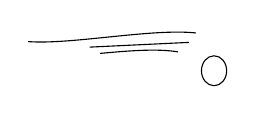
\begin{tikzpicture}[x=1cm,y=1cm]
\draw (0,.26)..controls (.55,.22) and (1.57,.43)..(2.13,.37);
\draw (.78,.19)--(2.04,.25);
\draw (.91,.11)..controls (1.34,.15) and (1.65,.17)..(1.90,.13);
\draw (2.36,-.11) ellipse (.16 and .19);
\end{tikzpicture}}

Soit $\Lambda$ une algèbre $k$-augmentée dont l'idéal
d'augmentation est \deleted{nilpotent}\inserted{de puiss. n.ième nulle}, $k$ étant une
algèbre contenant $\mathbb Q$\inserted{[donc $\Lambda$ contient $\mathbb Q$]}, Soit $M$ un $\Lambda$-module.
Alors les $u\in L_\Lambda(M)$ tels que $uM\subset I(\Lambda)M$
\inserted{i.e. $u$ induit $0$ dans $M\otimes_\Lambda k$}
sont nilpotents \deleted{\unsure{et les sont}}\inserted{(de puiss. n:ième nulle)} les
$v\in L_\Lambda^{\unsure{*|\times}}(M)$ tels que $v$ induise l'identité
dans $M\otimes_\Lambda k$ sont unipotents ; si \unsure{l'ens|l'ens.}
des uns et des autres est $\unsure{\pi^\ell_a|\pi_a}$ resp$^{\mathrm t}$ $\gamma$,
% archive sheet number: 13

